%%%%%%%%%%%%%%%%%%%%%%%%%%%%%%%%%%%%%%%%%
% CU Boulder Physics Lab Writeup One Column
% LaTeX Template
% Version 1.0 (2022-10-05)
%
% This template has been downloaded from:
% http://www.LaTeXTemplates.com
%
% Original author:
% Mathias Legrand (legrand.mathias@gmail.com) titled Stylish Article 
% With extensive modifications by:
% Vel (vel@latextemplates.com)
% Further modifications for CU Boulder Physics by:
% Kristopher Bunker (kristopher.bunker@colorado.edu)
%
% License:
% CC BY-NC-SA 3.0 (http://creativecommons.org/licenses/by-nc-sa/3.0/)
%
%%%%%%%%%%%%%%%%%%%%%%%%%%%%%%%%%%%%%%%%%

%----------------------------------------------------------------------------------------
%	PACKAGES AND OTHER DOCUMENT CONFIGURATIONS
%----------------------------------------------------------------------------------------

\documentclass[10pt]{PhysLab1C} % Document font size

\usepackage[english]{babel} % Specify a different language here - english by default


%----------------------------------------------------------------------------------------
%	COLUMNS
%----------------------------------------------------------------------------------------

\setlength{\columnsep}{0.55cm} % Distance between the two columns of text
\setlength{\fboxrule}{0.75pt} % Width of the border around the abstract

%----------------------------------------------------------------------------------------
%	COLORS
%----------------------------------------------------------------------------------------

\definecolor{color1}{RGB}{0,0,90} % Color of the article title and sections
\definecolor{color2}{RGB}{0,20,20} % Color of the boxes behind the abstract and headings

%----------------------------------------------------------------------------------------
%	HYPERLINKS
%----------------------------------------------------------------------------------------

\usepackage[pdfencoding=auto, psdextra]{hyperref} % Required for hyperlinks


\hypersetup{
	hidelinks,
	colorlinks,
	breaklinks=true,
	urlcolor=color2,
	citecolor=color1,
	linkcolor=color1,
	bookmarksopen=false,
	pdftitle={Title},
	pdfauthor={Author},
}

%----------------------------------------------------------------------------------------
%	LAB AND COURSE INFORMATION
%----------------------------------------------------------------------------------------

\CourseInfo{Electronics for the Physical Sciences \vert ~ \textbf{PHYS 3330}} %
\Department{\copyright \ Department of Physics \vert ~ \textbf{University of Colorado Boulder} \ \vert ~ \textbf{\today}} %
\Copyright{\today} %

\LabTitle{Modeling Measurement Systems Using Voltage Dividers} % Lab Title

%----------------------------------------------------------------------------------------
%	ABSTRACT
%----------------------------------------------------------------------------------------

\Abstract{\textbf{Lab 2:} Measuring properties of voltage dividers, developing models of
measurement devices (DMM, Scope), and building a variable voltage source}

%----------------------------------------------------------------------------------------

\begin{document}

\maketitle % Output the title and abstract box

%\tableofcontents % Output the contents section

\thispagestyle{firstpage} % Removes page numbering from the first page

%----------------------------------------------------------------------------------------
%	ARTICLE CONTENTS
%----------------------------------------------------------------------------------------

\section{Goals}

In this lab, you will gain experience working with the prototyping
board, which will be the main platform for building circuits for the
rest of the semester. You will also learn how to refine you model of a
circuit to include the measurement probes. Finally, you will use apply
your knowledge of voltage dividers to build a dimmer switch.

Proficiency with new equipment:

\begin{itemize}
\item
  Prototyping board:

  \begin{itemize}
  \item
    Set power rails on the board
  \item
    Determine the connection layout on the proto-boards
  \item
    Be able to assemble resistive circuits and measurement test points
    on the boards
  \end{itemize}
\item
  Potentiometers

  \begin{itemize}
  \item
    Determine the connections on a 10-turn pot
  \item
    Use a pot to continuously control an output voltage
  \end{itemize}
\end{itemize}

Modeling measurement systems:

\begin{itemize}
\item
  Develop mathematical and schematic models of voltage dividers
\item
  Refine the voltage divider models to include the effect of the
  measurement probes
\end{itemize}

Applications

\begin{itemize}
\item
  Build a dimmer switch for a light bulb
\end{itemize}

%------------------------------------------------

\section{Definitions}

\textbf{Potentiometer (pot)} - a three-terminal resistive device that
provides a variable resistance between the ends and the "wiper"
connection.

%------------------------------------------------

\section{Useful Readings}

\begin{enumerate}
\item
  \href{https://atomoptics-nas.uoregon.edu/~dsteck/teaching/electronics/electronics-notes.pdf}{Steck}
  Sections 1.3.3 - 1.4.2
\item
  Fischer-Cripps Sections 2.1 - 2.3
\item
  Horowitz \& Hill 2\textsuperscript{nd} Ed. Sections 1.03 - 1.04
\end{enumerate}

%------------------------------------------------

\section{Prelab}

Answer the following questions in your lab notebook. Scan the relevant
pages and upload the PDF file. Note that the lab prep activities are
directly related to the lab and by completing them (and having them
available during lab) you will be able to work through the lab more
efficiently and be able to understand what you are doing during the lab.

\subsection{Resistive voltage dividers (ideal power supply)}

An ideal voltage source (no internal resistance) drives current around
the loop of resistors shown in Figure \ref{ideal-vd}.

\begin{enumerate}
 \item
  Derive a formula for the current, I, and the output voltage, $V_{out}$.
 \item
  What is $V_{out}$ if $V = 10~V$, $R_{1} = 2~k\Omega$, and $R_{2} = 1~k\Omega$?
 \item
  Calculate the voltage $V_{out}$ for the modified circuit
  shown in Figure \ref{modified-vd} with $R_{3} = 10~k\Omega$ and the other
  components unchanged.
\end{enumerate}

\subsection{Resistive voltage dividers (non-ideal power supply)}

A non-ideal voltage source has an output impedance (resistance). First
consider a supply with an output impedance 500 $\Omega$.

\begin{enumerate}
\def\labelenumi{\arabic{enumi}.}
\item
  Draw a modified circuit diagram of Figure \ref{ideal-vd} to model the non-ideal
  voltage source as an ideal source with a series resistor.
\item
  Derive a formula for the current, I, and the output voltage,
  V\textsubscript{out} of the circuit you just drew.
\item
  What is V\textsubscript{out} if V = 10 V, R\textsubscript{1} = 2 k$\Omega$,
  and R\textsubscript{2} = 1 k$\Omega$ ?
\item
  An additional load is connected between V\textsubscript{out} and
  ground in the form of the resistor R\textsubscript{3} as shown in
  Figure \ref{modified-vd}. Calculate the voltage V\textsubscript{out} for this
  circuit (with the non­‐ideal power supply) and with R\textsubscript{3}
  = 10 k$\Omega$.
\item
  Using your symbolic equation for V\textsubscript{out}, solve for
  R\textsubscript{3}. (This will be super helpful for use in the lab).
\end{enumerate}

\subsection{Lab activities}

% \begin{enumerate}
% \item
%   Read through all of the lab steps and identify the step (or sub-step)
%   that you think will be the most challenging.
% \item
%   List at least one question you have about the lab activity.
% \end{enumerate}

% \begin{figure}[h]
% \centering
% \begin{subfigure}[t]{0.3\textwidth}
% \centering
% \begin{circuitikz}[american voltages]
% \draw (0,0)
%     to [V, invert, *-, l=$V$] (0, 4) %-- ++(2,0)
%     to [short, f=$I$] ++(2,0)
%     to [R=$R_1$, -*] ++(0,-2)
%     to [R=$R_2$, -*] ++(0,-2)--(0,0) node[ground]{};
%     \draw (2,2) to [short, -o] (4,2) node[anchor = west]{$V_{out}$};
%     \draw (2,0) to [short, -o] (4,0) node[anchor = west]{$0~V$};
% \end{circuitikz}
%  \caption{}
%  \label{ideal-vd}
%  \end{subfigure}
%  \hspace{1.1cm}%
%  \begin{subfigure}[t]{0.3\textwidth}
%  \centering
% \begin{circuitikz}[american voltages]
% \draw (0,0)
%     to [V, invert, *-, l=$V$] (0, 4) %-- ++(2,0)
%     to [short, f=$I$] ++(2,0)
%     to [R=$R_1$, -*] ++(0,-2)
%     to [R=$R_2$, -*] ++(0,-2)--(0,0) node[ground]{};
%     \draw (2,2) to [short, -o] (4.5,2) node[anchor = west]{$V_{out}$};
%     \draw (2,0) to [short, -o] (4.5,0) node[anchor = west]{$0~V$};
%     \draw (3.5,2) to [R=$R_3$, *-*] ++(0,-2);
% \end{circuitikz}
%  \caption{}
%  \label{modified-vd}
%  \end{subfigure}
%  \caption{Voltage Dividers}
%  \end{figure}

 
%  \begin{figure}[h]%
%     \centering
%     \subfloat[\centering Ideal Voltage Divider]{{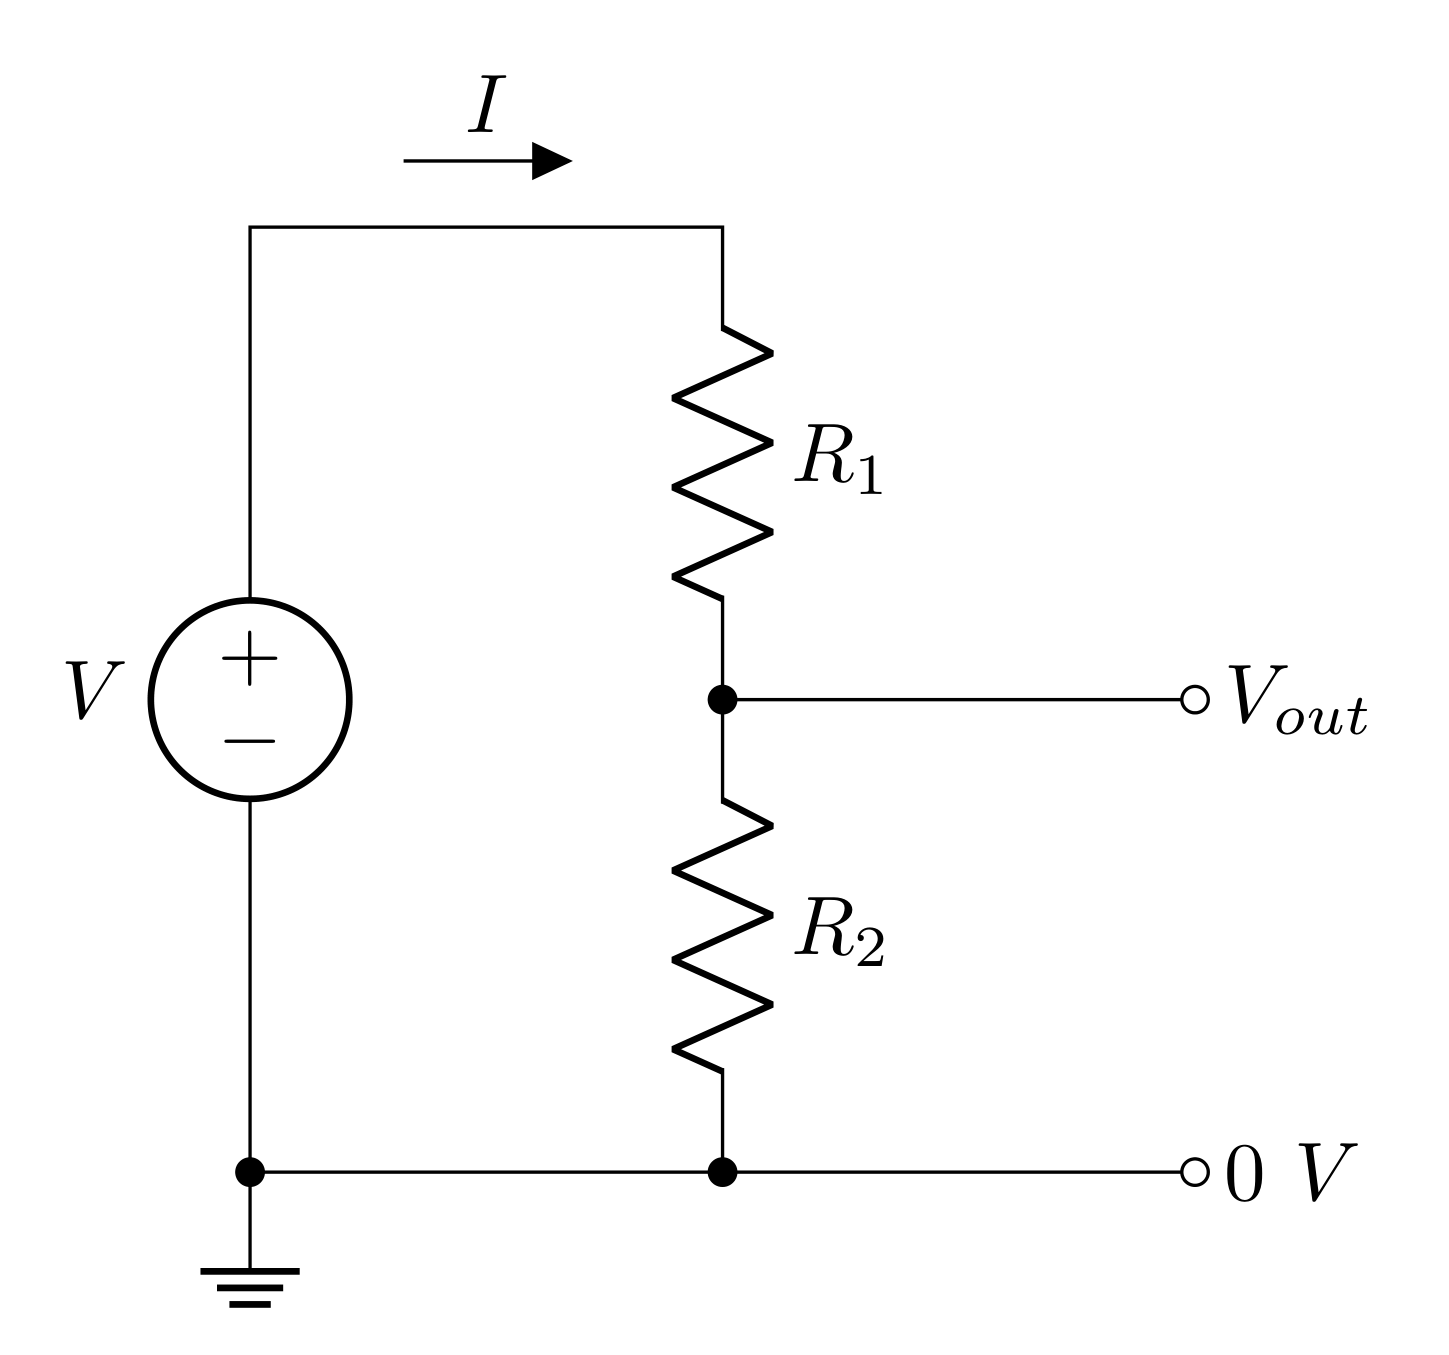
\includegraphics[height=6cm]{lab2fig/ideal-vd.png} } \label{ideal-vd}}%
%     \qquad
%     \subfloat[\centering Modified Voltage Divider]{{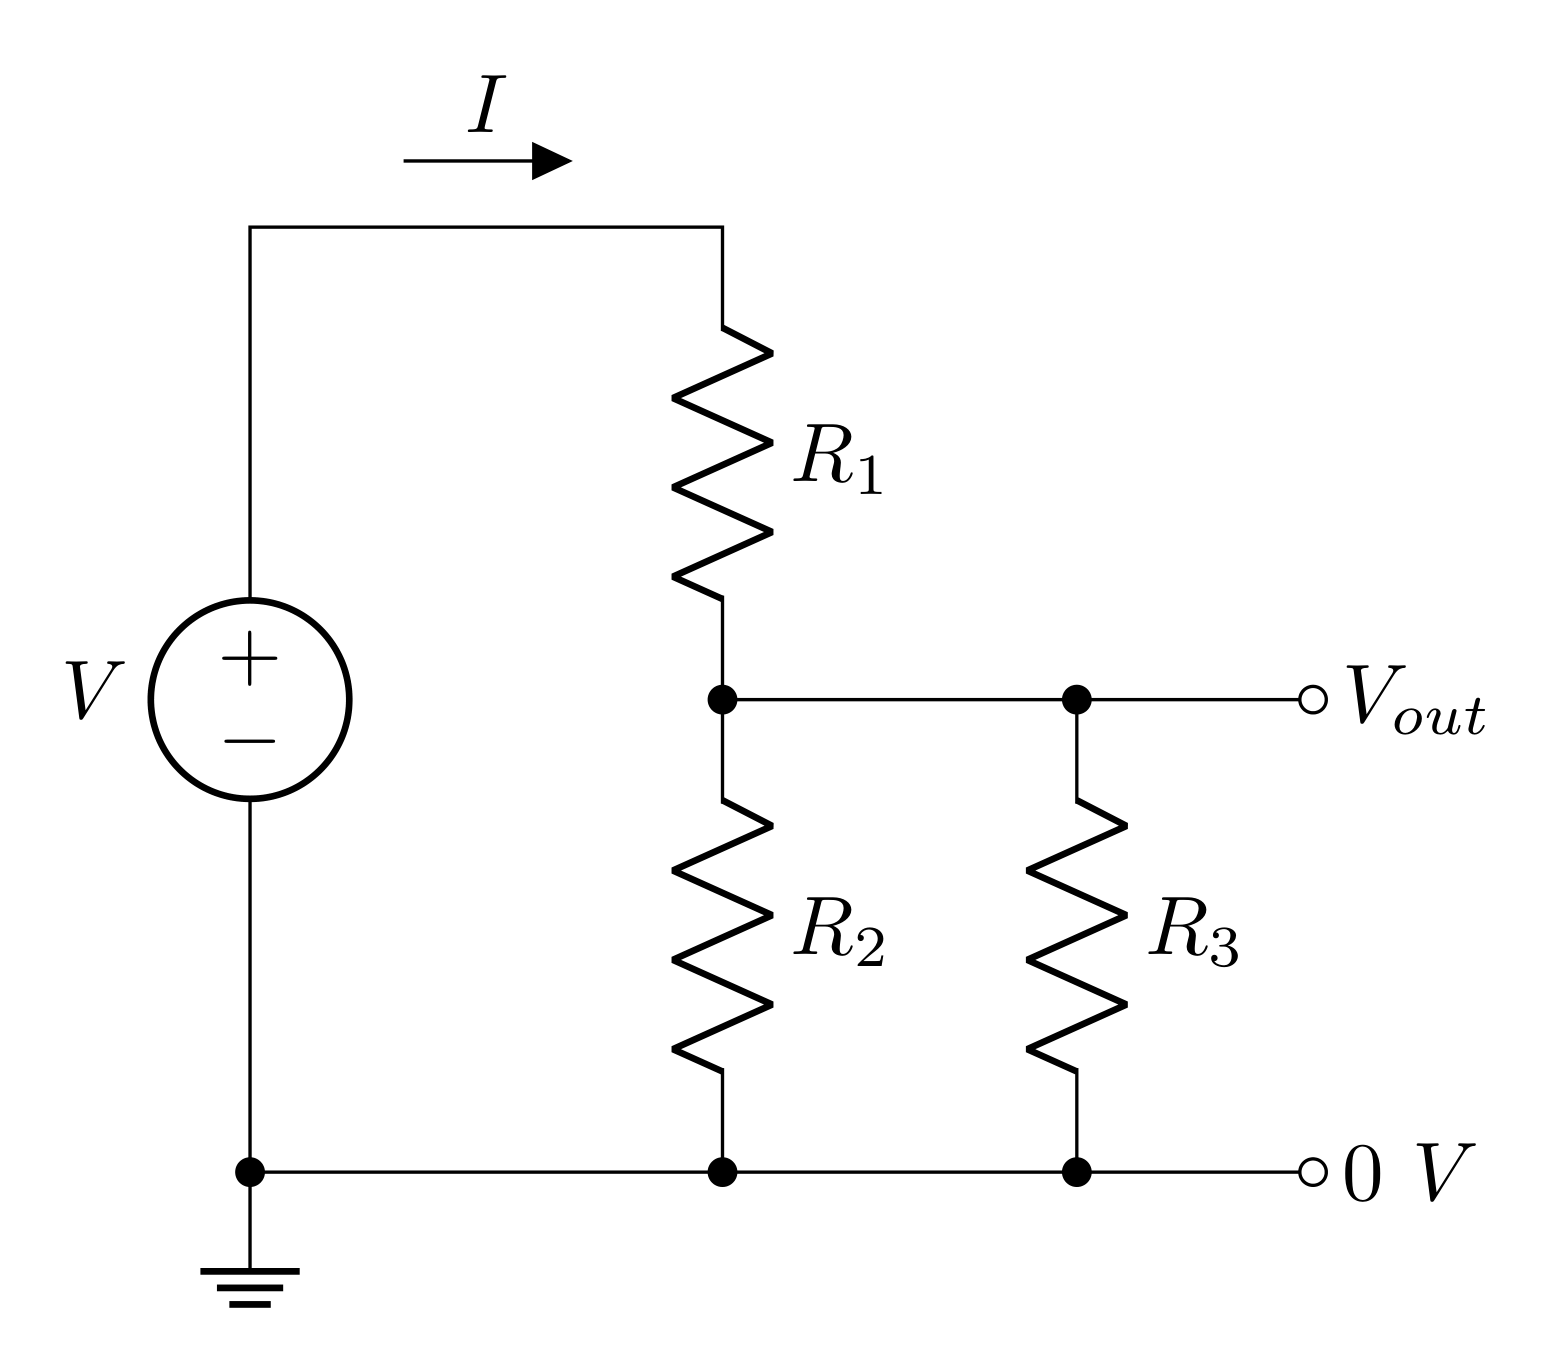
\includegraphics[height=6cm]{lab2fig/modified-vd.png} }\label{modified-vd}}%
%     \caption{Voltage Dividers}%
%     \label{fig:bnc}%
% \end{figure}

\begin{figure}[h]
     \centering
     \begin{subfigure}[b]{0.4\textwidth}
         \centering
         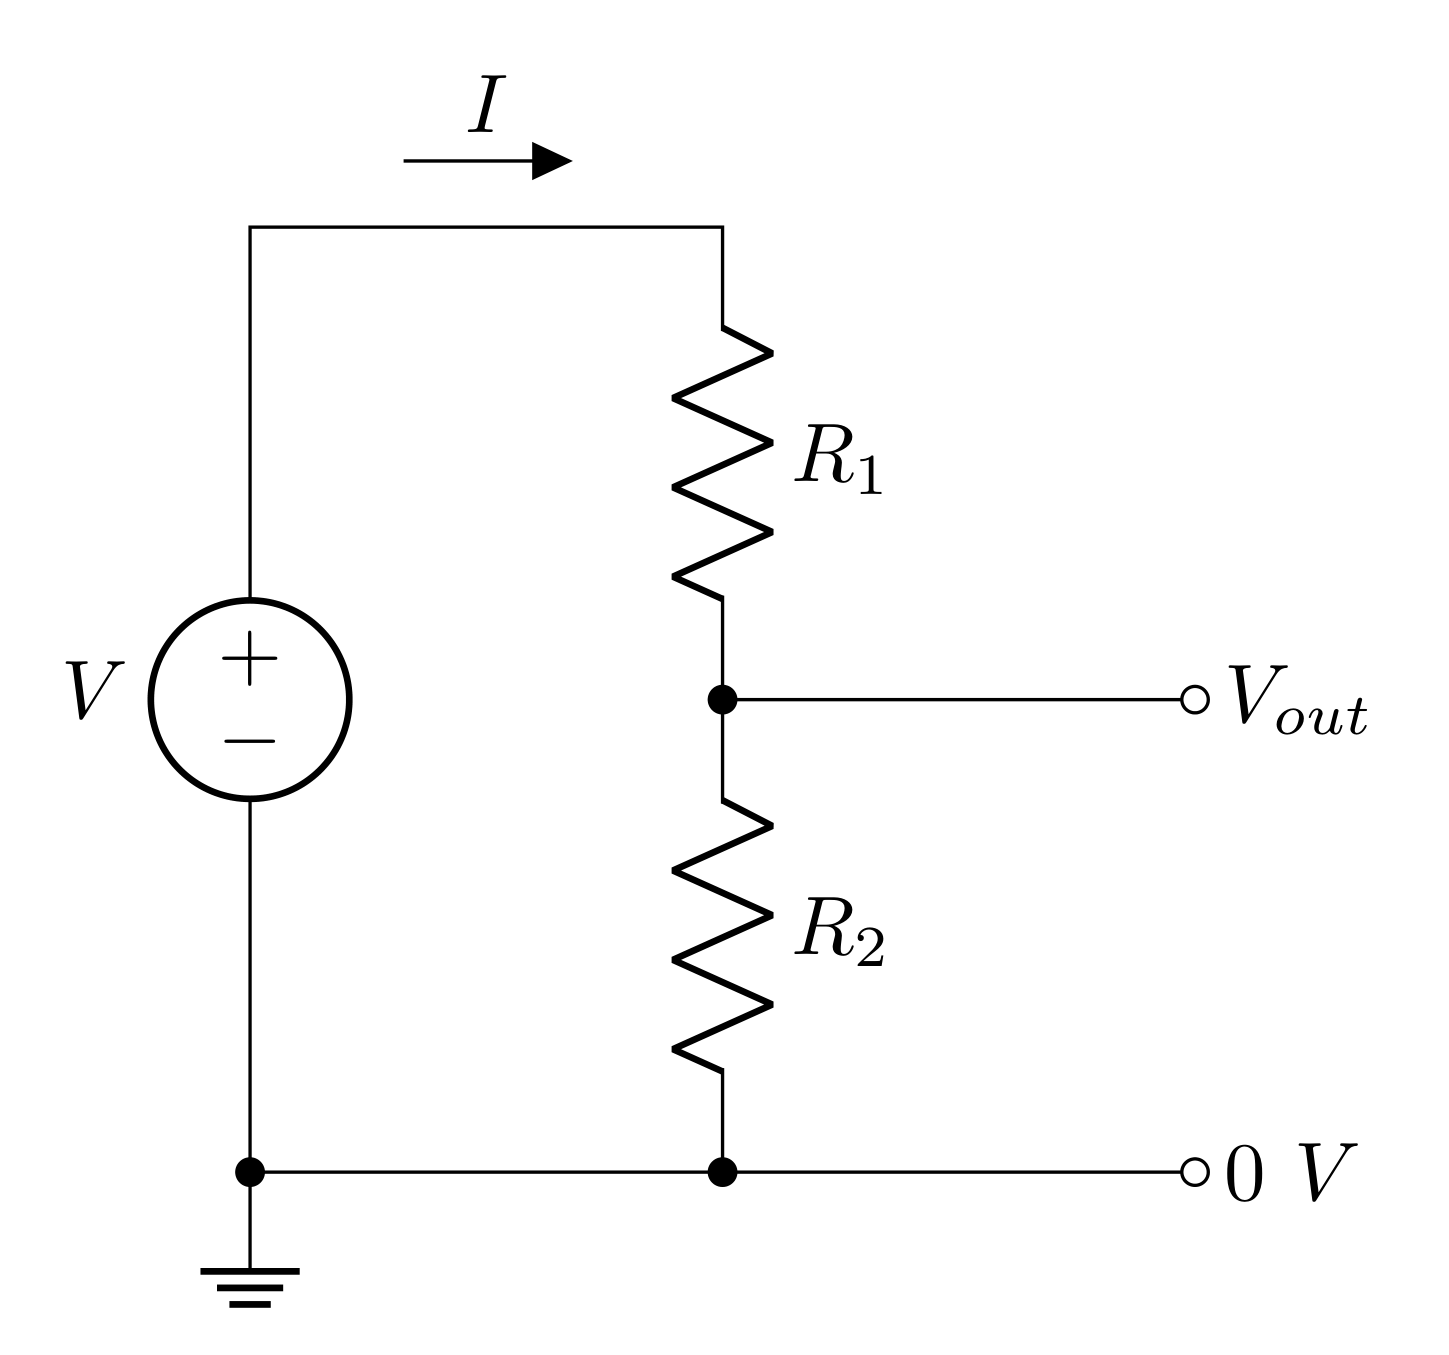
\includegraphics[height=5cm]{lab2fig/ideal-vd.png}
         \caption{Ideal Voltage Divider}
         \label{ideal-vd}
     \end{subfigure}
     %\hspace{2cm}
     \begin{subfigure}[b]{0.4\textwidth}
         \centering
         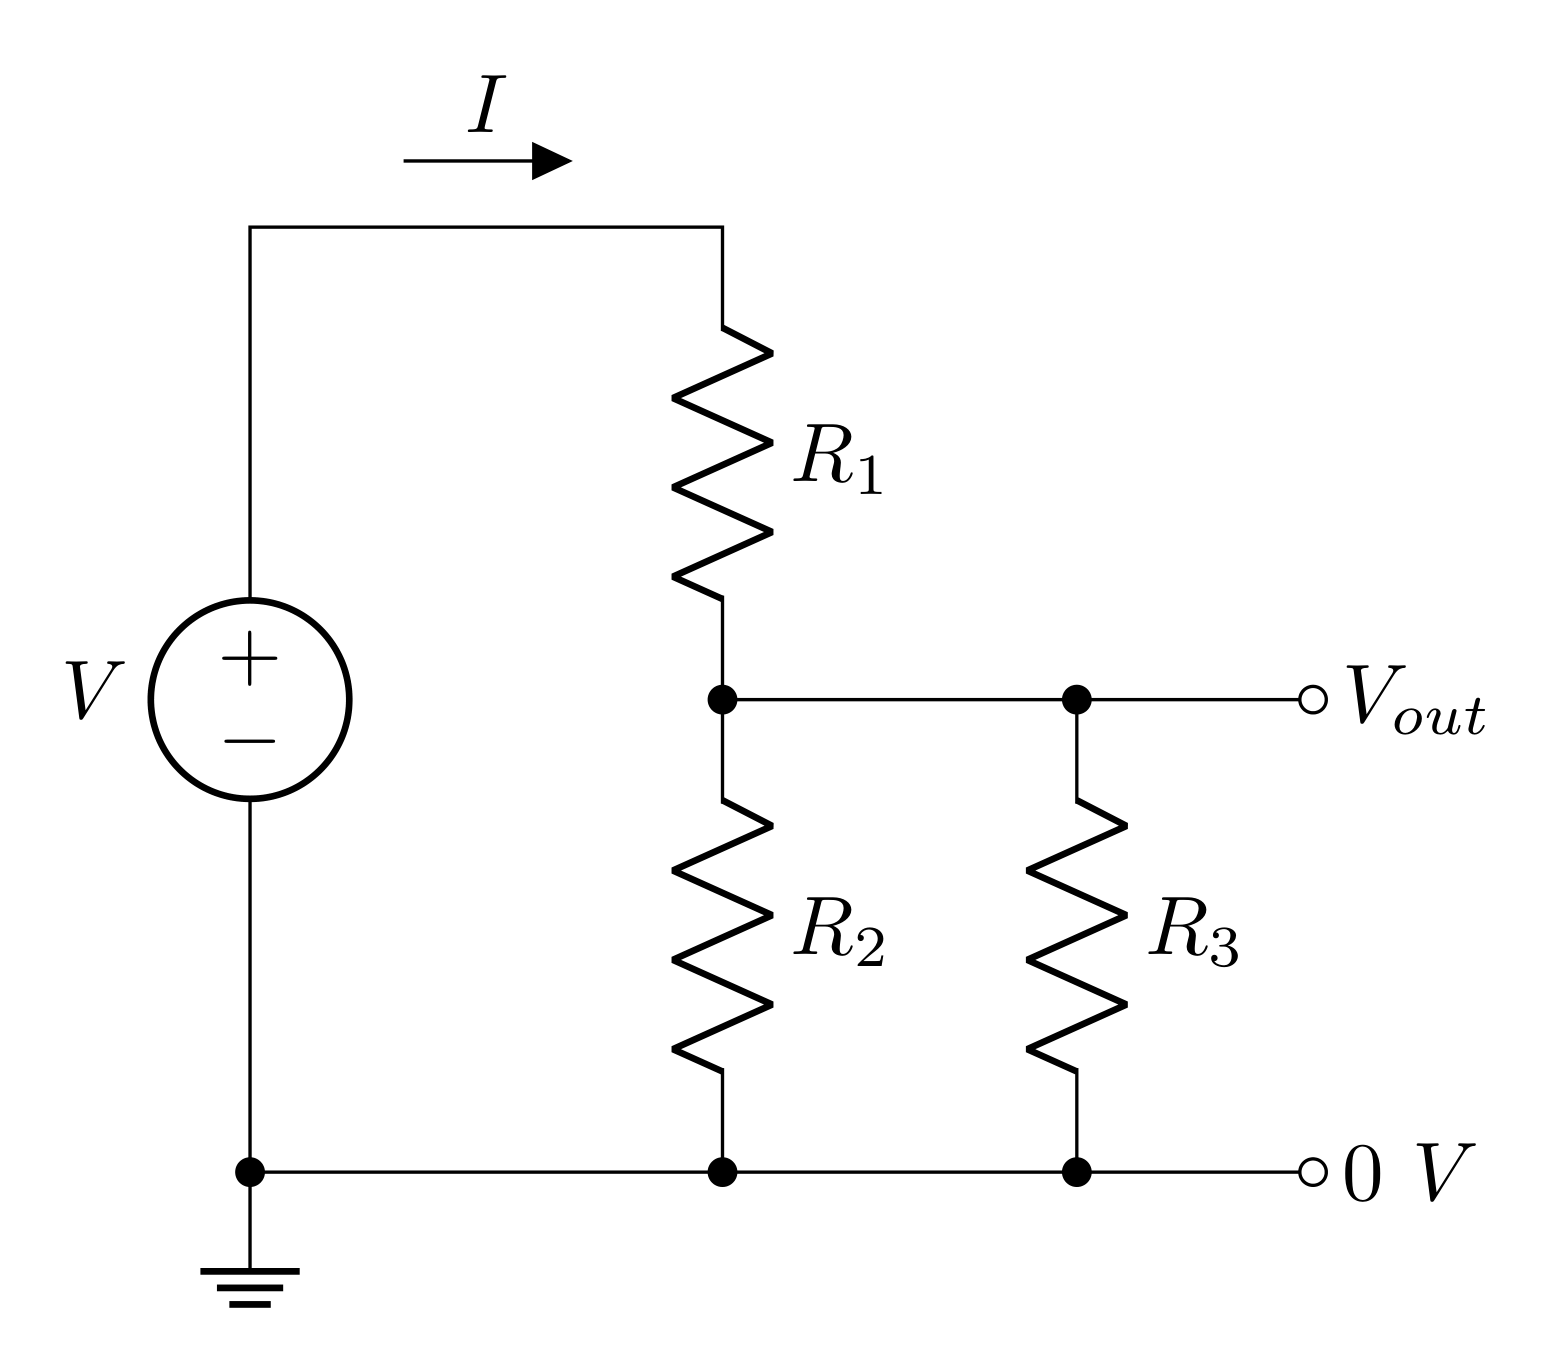
\includegraphics[height=5cm]{lab2fig/modified-vd.png}
         \caption{Modified Voltage Divider}
         \label{modified-vd}
     \end{subfigure}
     \medskip
        \caption{Filters}
        \label{fig:bnc}
\end{figure}



%------------------------------------------------

\section{Setting Up Your Prototyping Board}

Before breadboards (aka prototyping or proto boards), creating circuits
required soldering all components together, and changing the circuit was
difficult. Breadboards allow for quickly creating and modifying
circuits, with no soldering. Once the circuit works and meets the
desired specifications, the circuit can be built using more permanent
methods such as soldering to a Vector board or to a printed circuit
board. Present technology allows anyone to cheaply design, layout, and
print professional circuit boards. For example:
\url{http://www.expresspcb.com/}

\subsection{Test your protoboard}

\begin{enumerate}
\def\labelenumi{\arabic{enumi}.}
\item
  Your instructor will give your team a prototyping board to use. Write
  your team member\textquotesingle s names on it. Your team will use the
  same board all semester. An incomplete experiment can be left on the
  board and finished later. Store the board on the shelf labeled for
  your section.
\item
  On the front panel, you will find:

  \begin{itemize}
  \item
    \underline{BNC cable jacks} that carry electric signals between your
    circuit on the board and the function generator and oscilloscope
  \end{itemize}

  \begin{itemize}
  \item
    \underline{Colored banana jacks} to bring in DC power for transistors or
    chips from an external power supply
  \end{itemize}

  \begin{itemize}
  \item
    A precision 10 k$\Omega$ ten‑turn \underline{potentiometer}
  \end{itemize}

  \begin{itemize}
  \item
    Several \underline{switches}
  \end{itemize}

  A wire or component on the board might be broken, or might break
  during the semester. Don\textquotesingle t worry -you will be able to
  repair the board as you go.
\item
  The breadboard contains arrays of holes, interconnected by buried
  conductors, into which components are plugged to build your circuit.
  In general, you can never be sure that any two contacts are really
  connected, or any wire is really continuous, unless you test it
  yourself, so get into the habit of testing things.
\item
  Determine which holes on your protoboard are connected by using the
  DMM (you may also find wires and alligator clips useful). Draw a
  diagram in your lab notebook of the connections. You can refer back to
  this diagram throughout the semester as you build new circuits.
\item
  Find a 1k resistor and measure the resistor directly with the DMM. Now
  insert the resistor into two holes on the breadboard that you know are
  not connected and remeasure the resistance. Now insert the resistor
  into two holes on the breadboard that you know \textbf{are} connected
  and remeasure the resistance. Explain your results. What does this
  tell you about when you should measure resistors?
\end{enumerate}

\subsection{Making power connections to your protoboard}

\begin{enumerate}
\def\labelenumi{\arabic{enumi}.}
\item
  For essentially all circuits, you will need power connections (+15 V,
  -15V, ground). Connect the power supply to the panel using banana
  cables.
\item
  \textbf{USE A COLOR CODE FOR THE POWER CONNECTIONS!} Typically we use
  \textbf{black = ground}, \textbf{\color{red}red = +15 V}, and \textbf{\color{blue}blue = -15
  V}. Using a consistent color code will allow you and others to debug
  your circuits quickly. You are also less likely to plug something in
  incorrectly and burn up a component. Write down your color code in
  your lab notebook.
\item
  Once you have power connected to the front panel, use the wires
  soldered on the back of the connectors to make connections to the
  board (+15, -15, and ground). The long rails that run the length of
  the board are best for distributing power to all of your components.
  Use these for only power or ground.
\item
  Good electrical contact is essential when you plug in components or
  wires. Use only 22- or 24-gauge solid wire, not stranded wire. The 22-
  or 24-gauge wire should make a good connection with the conductors
  inside the board without slipping out easily. Push in each wire until
  you feel the contacts grip. \textbf{Don\textquotesingle t force larger
  wires into the protoboard. You can damage the connectors.}
\item
  Reliable ground connections (0 V), readily accessible from any point
  on the board, are essential to the good functioning of most circuits.
  The front panel is the ground for your circuit board since the outside
  of the BNC connector connects the front panel of your circuit board to
  the ground of other instruments in your experiment.
\end{enumerate}

\subsection{Supplying power to your protoboard}

\begin{enumerate}
\def\labelenumi{\arabic{enumi}.}
\item
  Turn on your DC power supply such that it produces +15 V and -15 V.
  Set the current limit to about 100 mA. This will reduce the amount of
  smoke released from your components when you happen to plug in the
  power incorrectly. Describe the procedure you followed to set the
  current limit.
\item
  Measure the voltage on your protoboard rails using a DMM. You may need
  to use a wire to probe the voltage if your DMM probes do not fit in
  the holes. Always remember to measure voltages with respect to ground.
  Record the voltages in your lab notebook.
\end{enumerate}

%------------------------------------------------

\section{Building and Testing Voltage Dividers}

Components (resistors, capacitors, transistors, etc.) are
available from the community stock. Take what components you need for your experiments.

\subsection{Fixed-value voltage divider - 1k\texorpdfstring{$\boldsymbol{\Omega}$}{ohm}}

\begin{enumerate}
\def\labelenumi{\arabic{enumi}.}
\item
  Build a voltage divider similar to the one shown in Fig. 1(a) using
  resistors of around 1 k$\Omega$. Draw a diagram of the circuit in your lab
  notebook. Make sure to label the resistors and record all measured
  component values and voltages.
\item
  Measure each resistor with your DMM before inserting it into your
  circuit and record the value. Why should you measure component values
  before placing them in the circuit?
\item
  Predict the output voltage you should measure based on your input
  voltage and resistance measurements. Include your calculations and
  numerical predictions in your lab notebook.
\item
  Now, apply a DC voltage to the input and measure the output voltage of
  your divider, first using first your DMM and second using your
  oscilloscope with the minigrabbers. Record your measurements. \emph{Do
  not have the DMM and the oscilloscope connected at the same time
  because each may perturb the measurement differently.}
\item
  Compare the voltages you predicted to the voltages you measured. Does
  your model of the voltage divider agree with each of your
  measurements? Explicitly record what criteria you used to determine
  whether or not the model and measurements agreed.
\item
  \emph{Complete this step only if your model and measurements did not
  agree.} If your model and measurements did not agree, you will have to
  either refine your model or your experiment. Let\textquotesingle s
  start by refining your model. Consider the input resistance of your
  measurement device. Draw a circuit diagram that includes that
  resistance. \emph{HINT: See Fig. 1b.} Derive an expression for the
  output voltage now including the unknown measurement device
  resistance. Use this new model to determine the input resistance of
  measurement device. (that is, rearrange your equation to solve for
  R\textsubscript{3}). You may have this from your prelab.
\end{enumerate}

\subsection{Fixed-value voltage dividers of 1M\texorpdfstring{$\boldsymbol{\Omega}$}{ohm} and 10M\texorpdfstring{$\boldsymbol{\Omega}$}{ohm}}

\begin{enumerate}
\def\labelenumi{\arabic{enumi}.}
\item
  Complete the steps in the previous section for two additional voltage
  dividers, one using resistors 1M$\Omega$ and one with
  resistors 10M$\Omega$.
\item
  Using your refined model, you have determined the input resistance of
  both the DMM and scope. Specification (spec) sheets or data sheets can
  also be used to refine your model.
\item
  Look up the input resistance of your DMM using the spec sheets on
  Canvas. Does the measured input resistance agree with the instrument
  specs? Explicitly record what criteria you used to determine whether
  or not the resistances agree.
\item
  There is an easy way to determine the specified input impedance of the
  scope. Where can you find that information? Does the measured input
  resistance agree with the instrument specs? Explicitly record what
  criteria you used to determine whether or not the resistances agree.
\end{enumerate}

%------------------------------------------------

\section{Build a Controllable Voltage Source (Dimmer Switch}

You will now use your skills with building and testing voltage dividers
to build a controllable voltage source using a potentiometer.

\subsection{Testing your potentiometer (pot)}

\begin{enumerate}
\def\labelenumi{\arabic{enumi}.}
\item
  Set the dial to some point between 0 and 1000, but not 500. Since you
  have a 10-turn, 10 k$\Omega$ pot, the resistance between the wiper and one of
  the terminals should be equal to the dial value multiplied by 10 $\Omega$.
  The resistance between the wiper and the remaining terminal should be
  the previous resistance subtracted from 10 k$\Omega$.
\item
  Use the DMM to measure the resistance between all possible pairs of
  connections. Determine which terminal corresponds to the wiper, and
  which terminals correspond to the \textquotesingle0\textquotesingle{}
  and \textquotesingle1000\textquotesingle{} ends of the dial. Test with
  a DMM at a few different dial settings to get the hang of it.
\item
  Draw a diagram of the pot including a model of the internal components
  and external connections using the resistance observations.
\end{enumerate}

\subsection{Build a variable voltage source / Using a pot to build a light bulb dimmer}


\begin{enumerate}
\def\labelenumi{\arabic{enumi}.}
\item
  Draw a circuit diagram that uses one pot to create a variable voltage
  divider.
\item
  Derive an expression for the output voltage based on the input voltage
  and the two resistances. Are both resistances independently variable
  or a function of the other?
\item
  Construct your voltage divider and use a scope to measure the output
  voltage. Do you need to include the scope input resistance in your
  model? Explain why or why not.
\item
  Predict the maximum and minimum output voltage (when the wiper is at
  one end and then the other).
\item
  Test your model by making measurements on the scope. Make sure to
  include the limits of the voltage source. Do your measurements agree
  with your predictions? Explicitly record what criteria you used to
  determine whether or not the model and measurements agree.
\item
  Now connect a low voltage light bulb to the output. You may need to
  increase the current limit on the power supply to see visible light.
  Do not exceed 500 mA or your pot may burn out. Describe qualitatively
  the brightness of the bulb as the pot knob is adjusted. What is the
  minimum voltage needed to see the light bulb turn on?
\item
  \textbf{Bonus question:} A good voltage source has very little (a few
  ohms) output resistance and thus very little power is dissipated in
  the supply. What is the output resistance of the circuit (including
  your power supply and external components) if it produces 10V? Would
  this circuit be good for creating a variable voltage source in the
  range of 5-10 V? HINT: Consider the power dissipated in the source.
  Explain using your diagram, model, and values of resistance.
\end{enumerate}
%------------------------------------------------

\section{Summary and Conclusions}

Write a two-paragraph summary in your lab notebook of what you learned
and any important takeaways.

%------------------------------------------------

\section*{Appendix A: Calibrating the 10-turn Potentiometer (If Needed)}

\addcontentsline{toc}{section}{Appendix: Calibrating the 10-turn Potentiometer (If Needed)} % Adds this section to the table of contents

\begin{enumerate}
\def\labelenumi{\arabic{enumi}.}
\item
  The potentiometer on the circuit board panel has three connections.
  Two of the connections are at opposite end of a resistor. The third
  connection is connected to a sliding "wiper."
\item
  Your potentiometer is actually a very precise device! You can control
  the intermediate resistances at the level of 0.1\% with a little care.
  To understand how, examine the dial on the potentiometer. It should
  have a window with a number in it, and a dial marked with a scale that
  goes from 00 to 99. The digit in the window increments with each full
  turn of the dial, so it represents the most significant digit of the
  setting number: if it says \textquotesingle3\textquotesingle{} in the
  window and the dial reads 55, then the setting is 355. For a 10-turn
  potentiometer such as yours, the dial should be able to run from 000
  to 1000 by turning the knob ten full turns.
\item
  First, check if your pot is already calibrated! Turn the knob
  counterclockwise until it stops. If the dial reads 000 in this
  position, your pot is calibrated.
\item
  If the dial reads something other than 000 in this position, do the
  following procedure:

  \begin{enumerate}
  \def\labelenumii{\arabic{enumii}.}
  \item
    Use a tiny Allen key to loosen the small set-screw on the side of
    the knob.
  \item
    Pull the entire dial off the panel.
  \item
    Turn the inner knob that remains on your panel counterclockwise
    until it stops.
  \item
    Turn the now-detached knob until the dial reads 000.
  \item
    Push the dial back onto the inner knob, rotating the outside of the
    dial (not the knob!) counterclockwise until it snaps in place
    against the panel and won\textquotesingle t rotate. The dial should
    still read 000. If it doesn\textquotesingle t, repeat the last three
    steps.
  \item
    Use the Allen key to tighten the set screw. Check the calibration
    again: the knob should stop at 000 and 1000.
  \end{enumerate}
\end{enumerate}

%------------------------------------------------

\end{document}